\documentclass[variant=courcework]{bsuir}

\faculty{компьютерного проектирования}
\departmentlong{инженерной психологии и эргономики}
\departmentshort{эргономики}
\manager{эргономики}
\worktitle{Создание сервиса поиска визуально схожих изображений в
неорганизованных коллекциях}
\workcode{БГУИР КР 1-58 01 01 002 ПЗ}
\titleright{Студент\\Руководитель}
\titleleft{Бородин А.Н.\\Кабариха В.А.}
\titlepageyear{2024}

\graphicspath{{./assets/}}

\begin{document}

\maketitle

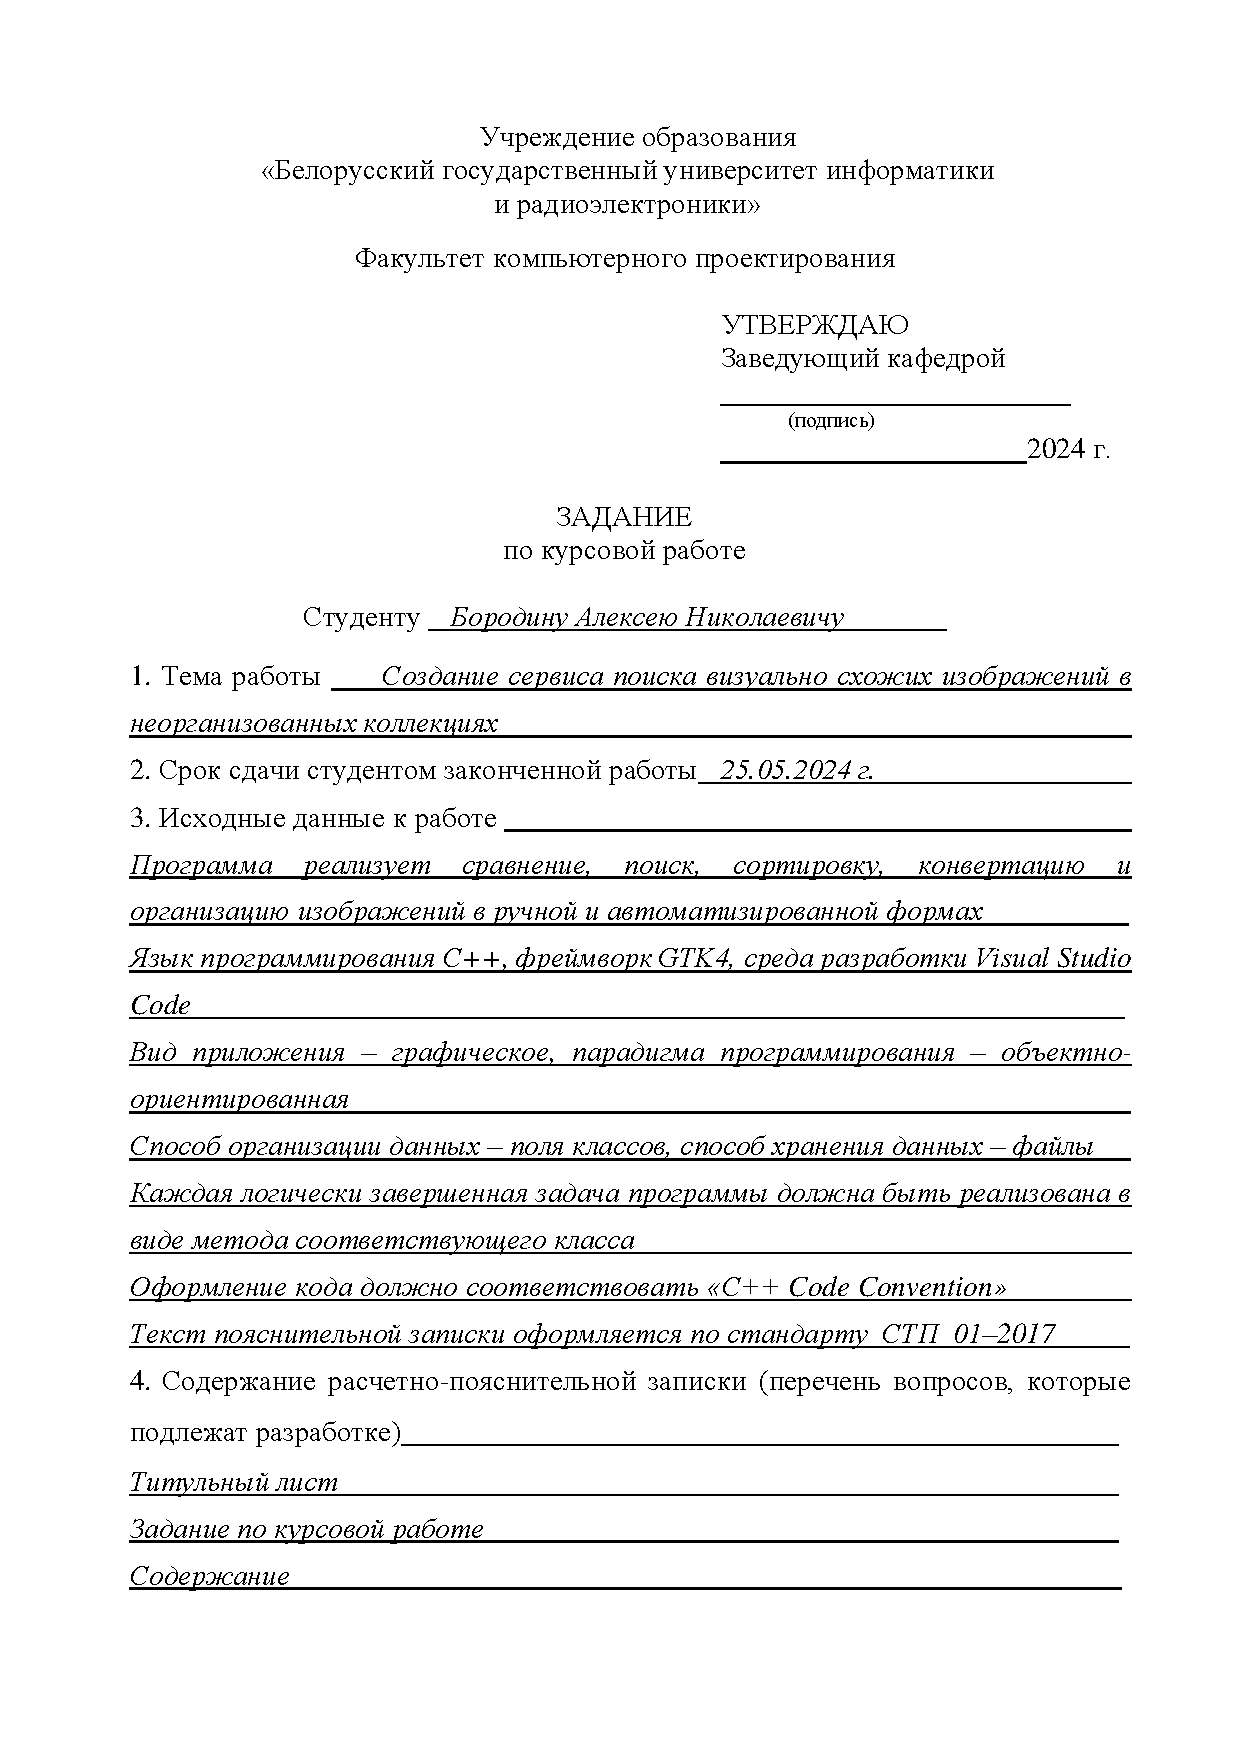
\includepdf[pages=-]{task.pdf}

\tableofcontents

\chapter*{Введение}

В современном мире объемы данных, включая изображения, растут с каждым днем.
Однако, с ростом количества данных возникает проблема поиска и классификации
информации. Визуальный поиск изображений становится особенно актуальным,
поскольку он позволяет пользователям находить изображения на основе их
визуальных характеристик, не зависимо от их текстового описания или тегов.

Сравнение изображений -- это процесс анализа двух или более изображений для
определения различий между ними. Это может включать в себя сопоставление
визуального содержания, такого как формы, цвета и текстуры, а также
использование алгоритмов для выявления изменений или аномалий. Сравнение
изображений широко используется в различных областях, включая цифровую
фотографию, медицинскую визуализацию, спутниковую разведку и системы
безопасности.

Целью данной курсовой работы является создание сервиса поиска визуально схожих
изображений в неорганизованных коллекциях на основе их визуальных характеристик,
таких как цвет, форма, текстура и других, даже если у них нет каких"=либо
метаданных, будь то теги или описание, который должен реализовать эффективную
систему индексации и хранения изображений, чтобы обеспечить быстрый доступ к ним
в коллекции и пользовательский интерфейс, который позволит пользователям
создавать выборки рассматриваемых файлов, следить за прогрессом сравнения и
просматривать результаты.

Данная работа будет включать в себя сравнительный анализ существующих решений,
оценочный выбор оптимальных инструментов для решения задачи, а также описание
разработанного сервиса. Будут представлены методы и алгоритмы, использованные
для сравнения изображений, описана система индексации и хранения данных, а также
представлен пользовательский интерфейс и результаты тестирования.

Ожидается, что результаты работы смогут применяться в реальных сценариях, где
требуется быстрый и точный поиск визуально схожих изображений в больших
коллекциях.

\chapter{Постановка задачи}

\section{Описание предметной области}

\subsection{Методики сравнения}
Визуальное сравнение изображений -- это процесс количественной оценки степени
визуального сходства между изображениями на основе извлекаемых из них
характеристик, с последующим ранжированием результатов. Можно выделить три
основных подхода к сравнению изображений: метрики структурного анализа,
хеширование изображений и использование машинного обучения.

\subsubsection{Метрики}
Метрика сходства -- это математическая абстракция для сравнения объектов,
присваивающая число, указывающее на степень родства между объектами указанной
пары \cite{ali2016survey}. Самый простой пример -- процент совпавших пикселей,
однако, существует множество более эффективных методов, различающихся по
сравниваемым признакам: цвет, текстура, форма и структура.

Метрики цвета количественно описывают распределение цветов и их статистические
характеристики в изображении. Чаще всего, речь о гистограммах. Гистограмма
изображения показывает частоту распределение пикселей различной интенсивности
показателя (цвет, освещенность и др.) \cite{ali2016survey}.

Метрики текстуры оценивают визуальные паттерны, структуру и неоднородности
поверхностей. Наиболее известны вейвлет"=преобразования. Вейвлет"=преобразование
одномерного сигнала состоит в его разложении по базису, сконструированному из
обладающей определенными свойствами солитоноподобной функции (вейвлета)
посредством масштабных изменений и переносов \cite{астафьева1996вейвлет}.

Метрики формы смотрят на геометрические и контурные особенности объектов.
Обычно, используются дескрипторы, такие как \textit{SIFT} (сравнение наборов
особых точек, найденных с помощью пирамиды гауссианов и ее разностей)
\cite{lowe2004distinctive}.

Наиболее популярны структурные метрики. Они позволяют оценить сходство
изображений по взаимосвязи между элементами. Каноничным примером алгоритма не
только структурного сравнения, но и визуального сравнения в целом считается,
имеющий десятки модификаций, \textit{SSIM} -- развитие методов \textit{RSNR} и
\textit{MSE}, с учетом специфики \textquote{восприятия ошибки}
\cite{wang2004image}.

\subsubsection{Хеширование}
Перцептивное хеширование -- отличается от метрики сходства наличием
промежуточного шага. Сравниваются не объекты, а их хеши. Операция сравнения
хешей проста и высокоэффективна, за счет чего можно значительно снизить
вычислительную нагрузку, если нужно сравнить эталон со множеством паттернов.
Вычисление всегда начинается с масштабирования изображения до маленького
размера, а затем проводится некоторое преобразование этой квадратной матрицы, в
зависимости от варианта алгоритма, за которым следует создание хеша из элементов
взятых в любом порядке. Для сравнения используют косинусное или Евклидово
расстояние или расстояние Хэмминга \cite{zauner2010implementation}.

Наиболее известны варианты основанные на дискретном косинусном преобразовании
(\textit{DCT}) для выделения низкочастотных компонентов (основной вариант,
Перцептивный хеш, \textit{pHash})\cite{zauner2010implementation}, на среднем
значении яркости (\textit{Average Hash}, \textit{aHash}), на основе блочного
среднего (\textit{Block Mean Hash}, \textit{bmHash}) и вейвлет"=функции
(\textit{Wavelet Hash}, \textit{wHash}) \cite{zauner2010implementation}.

\subsubsection{Машинное обучение}
Выделяется пять нейросетевых методов сравнения, которые позволяют извлекать и
сравнивать высокоуровневые визуальные признаки, что дает значительные
преимущества по сравнению с традиционными подходами. Они требуют несравнимо
больше аппаратных ресурсов чем метрики, однако гарантируют большую точность и
позволяют сравнивать смысловое содержание изображений: одинаковый ли объект (тип
объектов) на них изображен и на сколько они похожи.

Сети для извлечения дескрипторов обучаются извлекать компактные числовые
дескрипторы, описывающие визуальные характеристики изображений. Примером таких
сетей служит \textit{ResNet}\cite{simonyan2015deep}.

Сиамские нейронные сети состоят из двух или более идентичных подсетей, которые
обрабатывают несколько изображений параллельно; их обучают определять, являются
ли два изображения похожими или нет, на основе сравнения их внутренних
представлений \cite{koch2015siamese}.

Генеративные модели, например \textit{DCGAN}, могут сравнивать изображения на
основе их внутренних представлений \cite{radford2015unsupervised}.

Сети с контрастивным обучением используют методы контрастивного обучения для
различения похожих и непохожих изображений путем сравнения их внутренних
признаков, подобные \textit{SimCLR} \cite{DBLP:journals/corr/abs-2002-05709}.

Сети для семантической сегментации, такие как \textit{U-Net}, сравнивают
структуры и содержания на основе сегментированных областей
\cite{10.1007/978-3-319-24574-4_28}.

\subsection{Область применения}
Другой стороной предметной области является область применения. Сравнение
изображений находит широкое применение в различных сферах деятельности и
позволяет решать широкий спектр практических задач, связанных с анализом,
мониторингом и интерпретацией визуальной информации.

\subsubsection{Безопасность}
Одной из ключевых областей применения визуального сравнения изображений является
обеспечение безопасности и проведение наблюдения. Данная технология используется
для обнаружения изменений на охраняемых объектах, идентификации людей и
транспортных средств, мониторинга критической инфраструктуры, а также для
анализа видеонаблюдения в реальном времени с целью выявления аномалий и
подозрительной активности.

\subsubsection{Медицина}
В медицинской сфере визуальное сравнение изображений играет важную роль в
отслеживании прогрессирования или регрессии заболеваний, выявлении ранних
признаков патологий, оценке эффективности лечения, а также в автоматизированном
скрининге и диагностике на основе сравнения с базами данных типичных патологий.

\subsubsection{Промышленность}
Промышленность и производство также широко используют технологию визуального
сравнения изображений для контроля качества продукции, мониторинга
производственных процессов, отслеживания износа и повреждений оборудования, а
также для контроля качества упаковки и маркировки.

\subsubsection{Применение в быту}
Сравнение изображений применяется и в быту. Пользователи ищут по изображениям
именования заинтересовавших их предметов и желаемых товаров, местоположения
локаций и имена людей, изображенных на фотографиях, названия фильмов, передач и
сериалов по кадрам из них.

\subsubsection{Авторское право}
Кроме того, визуальное сравнение изображений находит применение в сфере
интеллектуальной собственности и авторского права. Эта технология используется
для поиска дубликатов и похожих изображений в больших базах данных,
классификации и каталогизации коллекций изображений, отслеживания использования
защищенных изображений в Интернете и выявления случаев плагиата.

\section{Сравнительный анализ}

\subsection{odiff}

\textit{odiff} -- консольная программа для сранения изображений. Она написана на
языке \textit{OCalm} и имеет привязку для использования в роли асинхронной
функции в \textit{nodejs}. Первый параметр вызова -- путь к эталонному
изображению, второй -- путь к изображению"=паттерну, с которым проводится
сравнение, а третий -- путь для записи результата сравнения. Само сравнение
проводится попиксельно и указывает красным цветом несовпадения. С заверения
разработчиков, программа в 6 быстрее ближайших конкурентов: \textit{pixelmatch}
и \textit{imagemagick compare} \cite{about-odiff}. Результаты работы изображены
на рисунке \ref{img:odiff}.

\makefigure{odiff}{
    \begin{subfigure}{.33\textwidth}
        \centering
        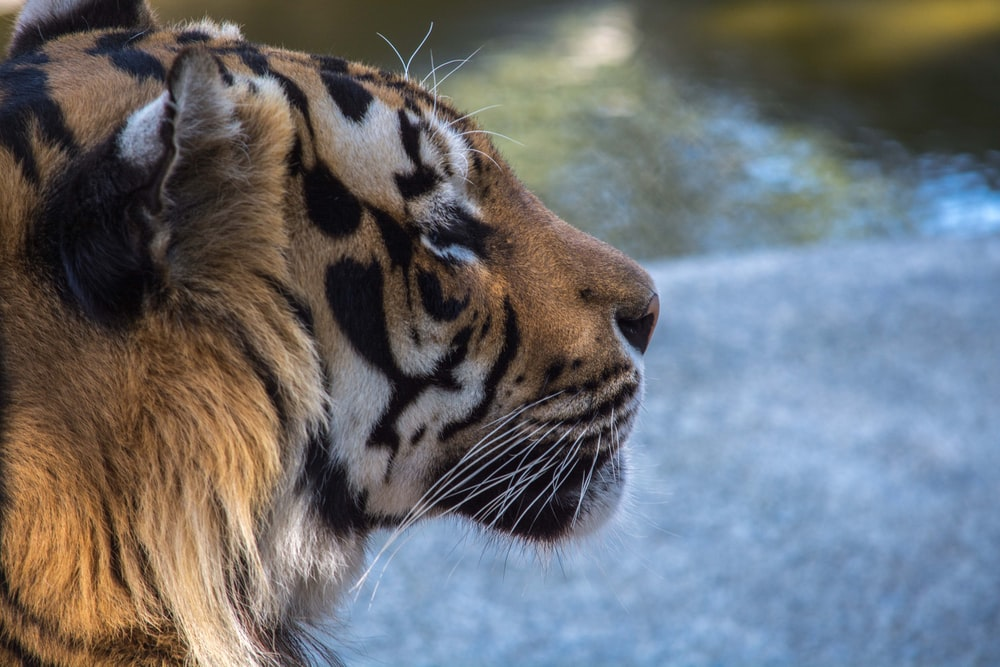
\includegraphics[width=.95\linewidth]{odiff1.jpg}
    \end{subfigure}%
    \begin{subfigure}{.33\textwidth}
        \centering
        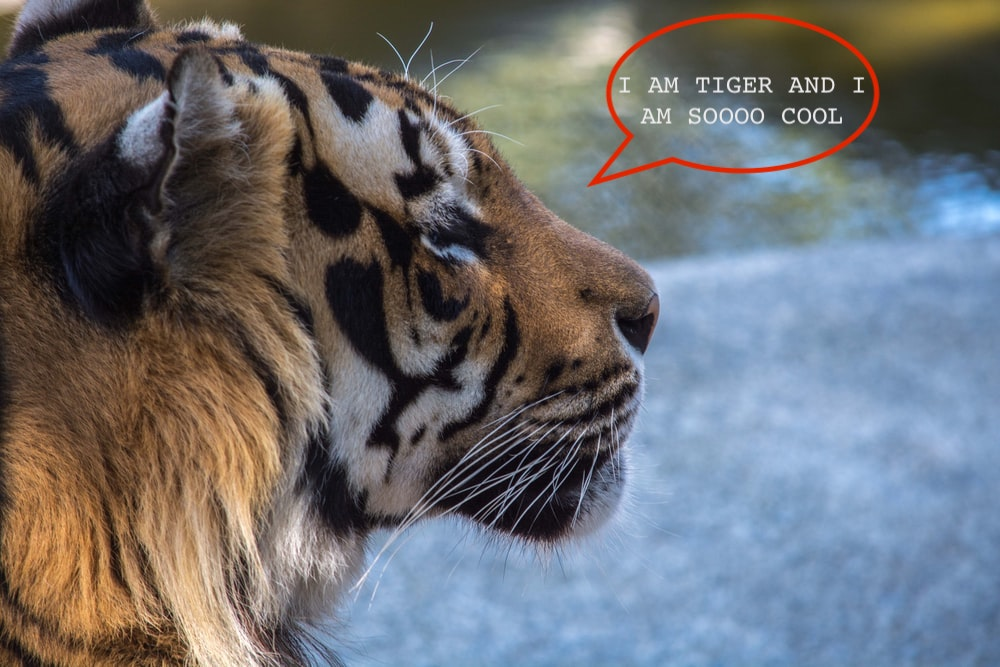
\includegraphics[width=.95\linewidth]{odiff2.jpg}
    \end{subfigure}%
    \begin{subfigure}{.33\textwidth}
        \centering
        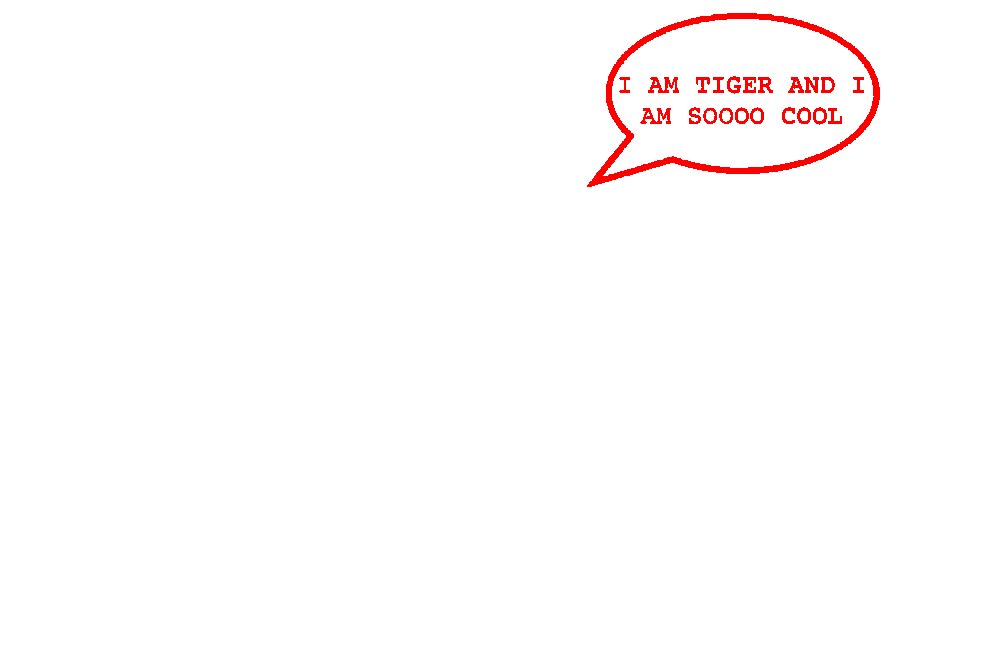
\includegraphics[width=.95\linewidth]{odiff3.png}
    \end{subfigure}
    \caption{Пример работы \textit{odiff}: эталон, паттерн, разница}
}

\subsection{ImageDeDup}
\textit{ImageDeDup} -- это библиотека на языке \textit{Python}, предназначенная
для поиска и удаления дублирующихся изображений. Она расчитана исключительно на
работу с изображениями и может быть встроена в другие программы или
использоваться непосредственно в роли утилиты в \textit{REPL}"=оболочке
\cite{about-imagededup}.

Библиотека предлагает несколько методов сравнения:

\begin{itemize}
    \item Сверточные нейронные сети (\textit{CNN}) -- использование готовых моделей
          или собственных.
    \item Перцептивное хеширование (\textit{PHash})
    \item Хеширование разностей (\textit{DHash})
    \item Вейвлет"=хеширование (\textit{WHash})
    \item Хеширование по средним значениям разностей (\textit{AHash})
\end{itemize}

\textit{ImageDeDup}, в первую очередь, ориентирована на исследовательские нужды
и работу с нейронными сетями, например, с использованием библиотек
\textit{NumPy} и \textit{Jupyter}. По"=этому она предоставляет возможность
генерации совмещенных изображений для иллюстрации результатов сравнения.

Для практического использования библиотека требует определенных навыков
программирования на \textit{Python}, так как код для выбора исходных файлов и
определения удаляемых дубликатов необходимо писать самостоятельно. На рисунке
\ref{img:imagededup.png} показан пример применения библиотеки для составления
сравнительного изображения для некоторого изображения со всеми в указанном
каталоге.

\makeimage[Пример применения \textit{ImageDeDup}]{imagededup.png}

\subsection{Czkawka}
Изображенная на рисунке \ref{img:czkawka.png}, \textit{Czkawka} -- наследница
заброшенного с 2017 года проекта \textit{FSlint}. В отличии от оригинала на
\textit{Python2/GTK+2} и работающего только под линукс-системами, разработан на
\textit{Rust/GTK4} (альтернативный фронтенд написан на \textit{slint}) и
кроссплатформенна. Программа обеспечивает широкий спектр интрументов для
поддержания порядка в файловой системе: помимо дедубликации посредством
универсального хеширования, имеются отдельные обработчики фото, аудио и видео,
поиск пустых и временных файлов и каталогов, невалидных ссылок и имен, больших
файлов. Для сравнение изображений используется настраиваемый перцептивный хеш
\cite{about-czkawka}.

Параметры перцептивного хеша:

\begin{itemize}
    \item Алгоритм масштабирования изображения: Lanczos3, ближайший сосед,
          треугольный, гауссовский, алгоритм Катмалла"=Рома;
    \item Размер хеша: 8, 16, 32, 64;
    \item Тип хеша: одинарный, вертикальный, двойной градиентный, блочный,
          средний.
\end{itemize}

\makeimage[Интерфейс \textit{Czkawka}]{czkawka.png}

\section{Информационная база задачи}

\subsection{Сводка}
Единственная информация, которую сервис сравнения изображений может хранить
между сеансами -- его конфигурация и, если еспользуется хеширование, кеш,
включающий в себя путь к файлу, его хеш и дату последнего изменения или иные
метаданные, сигнализирующие об изменении файла для пересчета его хеш"=суммы.
Форматы файлов выбираются в зависимости от фреймворка и вкусов разработчика. В
данной работе -- \textit{csv}.

\subsection{Местоположение}
Местоположение файлов конфигурации в \textit{linux}: \textit{/etc} для
общесистемных файлов и каталог, хранимый в переменной
\textit{\$XDG\_CONFIG\_HOME} или \textit{\$HOME/.config}, если таковой не
определено, для пользовательских параметров \cite{xdg_base_directory_spec}.

Кеш, если его сохраненность между перезапусками системы не требуется,
традиционно хранится в каталоге \textit{/etc}, иначе в
\textit{\$XDG\_CACHE\_HOME} или \textit{\$HOME/.local/}, если такового не
определено \cite{xdg_base_directory_spec}.

\section{Функциональное назначение}

\subsection{Загрузка изображений}
Программа должна поддерживать широкий спектр форматов изображений, включая
\textit{JPEG}, \textit{PNG}, \textit{WebP}, \textit{BMP} и другие.

\subsection{Просмотр списка}
Важной функцией является просмотр списка сравниваемых изображений. В нем должна
отображаться информация об изображении, такая как название, показатели схожести,
размер файла, формат, дата съемки или любые иные полезные для пользователя
метаданные.

\subsection{Фильтрация}
Важной функцией является поиска по изображениям и сортировка их списка по
метаданным, таким как название, описание, теги, дата съемки, дата сохранения,
местоположение.

\subsection{Сравнение изображений}
Ключевой функцией программ для сравнения изображений является возможность
открывать и отображать два или более изображения одновременно для визуального
сравнения.

\subsection{Экспортирование списка}
Для пользователя будет очень удобна возможность экспорта списка сравниваемых
файлов с указанием экспортируемых полей списка, формата и пути, по которому он
будет сохранен. Форматами могут служить: \textit{JSON}, \textit{YAML},
\textit{CSV} и другие. Также можно реализовать генерацию скриптов для выполнение
каких"=либо действий над списком. К примеру, удаление дубликатов с показателем
схожести выше 98 процентов.

\subsection{Поддерживаемые платформы}
Поддержка \textit{linux} как целевой платформы.\\

В разделе была рассмотрена задача о сравнение изображений, причины потребности
их сравнивать, существующие методы и программные решения. Помимо этого,
проведено их сравнение и оценена потребность в межсессионном хранении
информации, был составлен перечень требуемого функционала.

\chapter{Проектирование задачи}

\section{Алгоритм решения задачи}
% 2.1 Описываете способы решения задач, которые есть в приложении. Шифрование
% паролей, хранение информации, сортировка пользователей, создание интерфейса
% пользователя, описание проблем когерентности данных в файлах и способы их
% решения.

\subsection{Масштабирование изображения}
Сравнения изображений посредством перцептивного хеширования можно разделить на
три этапа: масштабирование изображений, вычисление хешей и их сравнение. Для
масштабирования изображения выбран алгоритм билинейной интерполяции, так как он
прост и эффективен. Он работает следующим образом: для каждого пикселя в новом
изображении находится ближайший пиксель в исходном изображении, а затем
вычисляется среднее значение цвета пикселей вокруг него. Этот метод обеспечивает
хорошее качество изображения при увеличении или уменьшении его размера.

\subsection{Вычисление хеша}
Перцептивное хеширование -- трехэтапный процесс

\subsection{Сравнение хешей}

\subsection{Обход коллекции}

\section{Логическое моделирование}
% 2.2 Описание модулей программы, каждый модуль описывается как самостоятельная
% единица, которая выполняет определённый набор функций в программе, нет
% ситуаций, когда модуль есть, чтобы есть. (Диаграмма классов)

\subsection{Модуль приложения}

\subsection{Модуль изображения}

\subsection{Модуль списка}

\section{Выбор и обоснование инструментов разработки}

\subsection{Язык программирования}
Сравнение изображений, как и любая операция над медиа"=данными, требует много
вычислений, что делает краеугольным вопрос оптимизации и производительности.
\textit{C++} заслуженно считается лидером по производительности, обычно
превосходя \textit{Rust} и не конкурируя с \textit{C}, будучи с ним совместимым
\cite{benchmarksgame}. \textit{Rust} более современный язык, стремящийся его
заменить, проигрывает в силу меньшей востребованности, из"=за чего, раз курсовая
работа выполняется в учебных целях, изучение \textit{C++} приоритетнее, а
\textit{C} и так его подмножество.

\subsection{Фреймворк}
Курсовая работа требует изучать новые технологии на ходу, из"=за чего, когда
зашла речь о выборе графического фреймворка \textit{GTK} был предпочтен более
сложному \textit{Qt}, реализующему свою вариацию \textit{STL}. В плане простоты
выигрывают \textit{WinForms} и \textit{wxWidgets}, однако, первый эксклюзивен
для \textit{Windows}"=систем, а второй, как и в случае с выбора языка,
проигрывает в популярности.

\subsection{Библиотеки}
В 2021 году, из"=за слишком сильной привязанности \textit{GTK} к \textit{GNOME},
было решено вынести ряд стандартных окон и форм в отдельную библиотеку,
названную \textit{Adwaita}, а в зависимости от того, используется ли она,
называться программы на \textit{GTK} \textit{GNOME}"= и
\textit{GTK}"=приложениями соответственно. В силу эстетической притягательности
форм, библиотека была подключена.

Реализация чтения и записи сложных форматов изображений, подобных \textit{PNG},
\textit{WebP} или \textit{AVIF} достойны быть темой отдельной курсовой работы, а
простые, такие как \textit{BMP}, не применяются на практике и сделают программу
бесполезной для конечного пользователя. Следовательно, решено использовать
библиотеку для работы с изображениями. \textit{Magick++} поддерживает больше
типов файлов, однако, за более удобное представление изображения в процессе
работы, предпочтена \textit{OpenCV}.

\subsection{Система сборки}
Для сборки проекта была использована комбинация \textit{Meson} и \textit{Nix}.
Первый -- рекомендованная разработчиками \textit{GTK} и \textit{GNOME}
современная декларативная система сборки, лучше адаптированная к \textit{GTK},
чем \textit{CMake} и в разы превосходящая слишком сложный, но малофункциональный
\textit{Autoconf}. Для установки зависимостей был использован \textit{nix},
пакетный менеджер с удобной функцией рабочих окружений в каталогах и
\textit{direnv} для их автоматической загрузки. Выбран, так как прост в
использовании, не засоряет систему дубликатами библиотек и не требует
дополнительной настройки для встраивания в цикл сборки, в отличии от
\textit{vcpkg}.

Для компиляции проекта использовался \textit{GCC}, так как, по неясным причинам,
только с ним заработало автодополнение кода в \textit{Visual Studio Code}, хотя,
планировалось использовать \textit{clang}, ведь использовались, зависящие от
него, \textit{clangd} и \textit{clang-uml}.

\subsection{Рабочая среда}
Для разработки программы был выбран редактор \textit{Visual Studio Code} по
следующим причинам:

\begin{itemize}
    \item Большой опыт его применения;
    \item Поддержка всех вышеназванных технологий через расширения, такие как
          \textit{clangd}, \textit{direnv}, \textit{Meson};
    \item За счет расширений формируется среда не только разработки программы,
          но и верстки пояснительной записки. Ключевая причина, так как
          воссоздать ее в другом \textit{IDE} будет тяжело.
\end{itemize}

В экосистеме \textit{GTK4} существует несколько способов разработки графического
интерфейса: программирование вручную, использование \textit{XML}"=описания,
\textit{blueprint}"=файлов или \textit{RAD}. Большинство разработчиков
предпочитают избегать описания интерфейса непосредственно в коде, так как это
приводит к избыточности и усложняет понимание программы. Использование
Декларативных \textit{XML} и \textit{blueprint}, также имеют свои недостатки, в
частности, громоздкость и проблемы с поддержкой некоторых функций
соответственно.

По"=этому, для проектирования пользовательского интерфейса был выбран
\textit{Cambalache} -- \textit{RAD}"=среда, пришедшая на смену устаревшему
\textit{Glade} и поддерживающая \textit{GTK4}.

% В конце раздела вывод по тому, что было сделано в разделе. 

% Для работы с дубликатами изображений наилучшим решением послужила программа,
% напоминающая файловый менеджер: выводящая список, считанных при запуске файлов
% текущего каталога, с возможностью его смены и просмотра файлов. Определение же
% дубликатов можно рассматривать как фильтр, исключающий все изображения, имеющие
% копию с большим или равным указанному значению процентом схожести. Также
% желательны было реализовать фильтр по имени файла и сортировку списка по
% наиболее важным параметрам при выборе копии, которая останется: местоположению,
% дате создания и размеру. Обладая выборкой файлов было бы естественно пожелать
% помимо возможности удалить ее, перенос, переименовывание или копирование.
% Особенно хорошо смотрелась бы конвертация файла в иной формат, при смене
% расширения и автоматическая очистка системы через автопоиск дубликатов и тихую
% конвертацию файлов в менее объемные форматы.

% В таком случае, каждую операцию над файлами и каждый фильтр можно реализовать
% как класс, соответствующий общему интерфейсу операции или фильтра, с которым
% работает класс списка, считывающий файлы каталога по данному ему пути и
% модифицирующий булевую маску видимости элементов исходя из переданной ему
% операции или же фильтра.

% \makesvg[Диаграмма вариантов использования]{usecases}







% Для решения задачи был выбран язык C++, как изучаемый и гарантирующий хорошие
% показатели производительности, а при работе с медиа это очень важный вопрос, и
% GTK, один из самых популярных фреймворков для построения графического
% интерфейса. Главным его конкурентом, обходящим по популярности, является Qt,
% который ориентируется на C++, пока GTK разрабатывается с расчетом на C.
% Контринтуитивно, однако был выбран GTK, ведь библиотеки на C проще адаптировать
% к другим языкам, из-за чего GTK можно использовать с любым популярным, или не
% очень, языком программирования, а так как разработчикам пришлость написать свою
% ООП--систему, а не влиться в существующую парадигму, его проще изучить.

% В мире GTK4 есть 4 способа разработки интерфейса: как код, XML, blueprint или в
% RAD. Большинство разработчиков предпочитают избегать описания интерфейса в коде,
% потому-что получается избыточно--многословно и усложняет понимания кода,
% рассредотачивая внимания и лишает дизайнеров шанса понять, что же делают
% разработчики. Для декларативного описания интерфейса используется местный
% безымянный диалект XML, но это язык не менее громоздкий, от чего был разработан
% blueprint-compiler, препроцессор, компилирующий QML--подобные blueprint--файлы в
% XML. Формат еще молод и имеет много проблем, к примеру, нет поддержки значений
% типа string[]. Следовательно, выбираем cambalache, RAD IDE, пришедшую на смену
% Glade, не поддерживающего GTK4.

% Для сборки проекта была использована комбинация meson и nix. Первый ---
% рекомендованная разработчиками GTK и GNOME система сборки, чьи дочерним проектом
% GTK и является, выгодно отличающаяся удобством использования и интеграцией с
% IDE, которая заставила отвернуться от классического для C++--проектов CMake и,
% тем более, свойственного малым Make. За счет интеграции, без проблем может быть
% использована любая IDE с поддержкой meson, такие, как Visual Studio Code. Nix
% же, как пакетный менеджер, отвечал за внешние зависимости проекта и
% пакетирование программы для полноценной ее установки.

% \chapter{Программная реализация}

% \section{Физическая структура}

% \subsection*{default.nix}

% Nix--пакет программы.

% \subsection{meson.build}

% Точка входа в систему сборки.

% \subsection{shell.nix}

% Конфиг рабочего окружения.

% \subsection{src/assets/logo/}

% Каталог с вариантами логотипа в разных размерах.

% \subsection{src/assets/meson.build}

% Скрипт сборки ассетов.

% \subsection{src/assets/template.desktop}

% Шаблон desktop--файла.

% \subsection{src/assets/template.desktop}

% Шаблон desktop--файла.

% \subsection{src/gresources.xml}

% Индекс всех ресурсов программы.

% \subsection{src/i18n}

% Каталог с файлами gettext--переводов.

% \subsection{src/main.cc}

% Точка входа в программу.

% \subsection{src/meson.build}

% Скрипт сборки программы.

% \subsection{src/views}

% Каталог с конфигурациями интерфейса.

% \section{Описание разработанных модулей}

% \subsection{Взаимодействие классов}

% \makesvg[Диаграмма классов]{classes}

% \subsection{main.cc}

% Инициализирует программу.

% \chapter{Тестирование}

% \chapter{Применение программы}

% \section{Руководство пользователя}

% \chapter*{Заключение}

\bibliography{lib}

\appendix

\chapter[обязательное]{Исходный код программы}

\makelisting{../src/application.cc}[src/application.cc]
\makelisting{../src/application.hh}[src/application.hh]
\makelisting{../src/gresources.xml}[src/gresources.xml]
\makelisting{../src/image.hh}[src/image.hh]
\makelisting{../src/list.hh}[src/list.hh]
\makelisting{../src/main.cc}[src/main.cc]
\makelisting{../src/main.hh}[src/main.hh]
\makelisting{../src/views/about.ui}[src/views/about.ui]
\makelisting{../src/views/application.ui}[src/views/application.ui]
\makelisting{../src/views/preferences.ui}[src/views/preferences.ui]

\chapter[справочное]{Код файлов конфигурации}

\makelisting{../meson_options.txt}[meson\_options.txt]
\makelisting{../meson.build}[meson.build]
\makelisting{../po/meson.build}[po/meson.build]
\makelisting{../src/assets/meson.build}[src/assets/meson.build]
\makelisting{../src/meson.build}[src/meson.build]

% \makeappendix{справочное}{Функция перцептивного хеша}{}

% \makeappendix[справочное]{Алгоритм обхода коллекции}{inventory.crop}

% \makeappendix{справочное}{Диаграмма деятельности}{}

% \makeappendix{справочное}{Диаграмма классов}{}

\makeappendix{Ведомость документов}{inventory}

\end{document}
